\subsection{Modeling}

\begin{frame}
  \frametitle{Model-Checking - Modeling}

  In MC we model the behavior of a system with the
  notion of {\bf state}. A state is a configuration of
  the system at a particular time instant 
  \vfill
  The system can change state by means of a {\bf transition}
  \vfill
  We are interested in a {\bf property} of the system
  \vfill
  \pause
  Example:
  \begin{itemize}
    \item System: a washing machine
    \item A state: ``the door is open and the engine is off''
    \item A transition: ``if the door is open then close the door''
    \item A property: ``When the engine is on, the door is closed''
  \end{itemize}

\end{frame}

\begin{frame}
  \frametitle{System to Model}

  \begin{center}
  
\includegraphics[scale=.67]{imgs/cheap-washing-machine-edit.png}
  \end{center}

\end{frame}

\begin{frame}
  \frametitle{Modeling - States}

  State variables can be used to describe a particular state
  \vfill
  \begin{center}
  \begin{tabular}{ll}
    \hline
    State variable & Values \\
    \hline
    door           & open, closed \\
    tray           & empty, filled \\ 
    engine         & off, on \\
    \hline
  \end{tabular}
  \end{center}
  \vfill\pause
  E.g.:
  \begin{center}
  \begin{tikzpicture}[auto]

%
% Styles
%
\tikzstyle{vertex} = [rectangle,draw=oproverblue!60,fill=oproverblue!20,thick]

\node[vertex] (x) at ( 0, 0)  {$\nodd{door=open}{engine=on}{tray=empty}$};

\end{tikzpicture}

  \end{center}
  which stands for ``the door is open, the engine is on, and the tray is empty''.\pause
  How many different states can we describe with our state variables ? 

\end{frame}

\begin{frame}
  \frametitle{Modeling - States}

  \begin{center}
  \begin{tikzpicture}[auto]

%
% Styles
%
\tikzstyle{state} = [rectangle,draw=oproverblue!60,fill=oproverblue!20,thick]
\tikzstyle{initialstate} = [rectangle,draw=mydarkgreen!80,fill=mydarkgreen!40,thick]

\node[initialstate] (000) at (  0,  -1)  {$\nodd{door=open}{engine=off}{tray=empty}$};
\node[state] (100) at ( -4, -2)  {$\nodd{door=closed}{engine=off}{tray=empty}$};
\node[state] (001) at (  4, -2)  {$\nodd{door=open}{engine=off}{tray=full}$};
\node[state] (101) at ( -2, -4)  {$\nodd{door=closed}{engine=off}{tray=full}$};
\node[state] (110) at (  2, -4)  {$\nodd{door=closed}{engine=on}{tray=empty}$};
\node[state] (011) at (  3, -6)  {$\nodd{door=open}{engine=on}{tray=full}$};
\node[state] (010) at (  0, -6)  {$\nodd{door=open}{engine=on}{tray=empty}$};
\node[state] (111) at ( -3, -6)  {$\nodd{door=closed}{engine=on}{tray=full}$};

\end{tikzpicture}

  \end{center}

  Some states are called {\bf initial} (green). Initial states 
  are the configurations of the system at time $0$

\end{frame}

\begin{frame}
  \frametitle{Modeling - Transitions}

  Transitions describe the evolution of the system. They transform
  the ``current'' state into a ``next'' state
  \vfill\pause
  \begin{center}
  \begin{tabular}{llllcl}
    \hline
    \multicolumn{4}{l}{Transition}   & ~~~ & Name \\
    \hline
    if & door=open  & then & door'=closed & & [close\_door] \\
    \\
    if & tray=empty & then & tray'=full   & & [fill\_tray] \\
    \\
    \multirow{2}{*}{if} & engine=off  & \multirow{2}{*}{then} & engine'=on  & & \multirow{2}{*}{[start\_wash]} \\ 
                        & door=closed &                       & tray'=empty & &                              \\
    \\
    \multirow{2}{*}{if} & \multirow{2}{*}{door=closed} & \multirow{2}{*}{then} & door'=open  & & \multirow{2}{*}{[open\_door]} \\ 
                        &                              &                       & engine'=off & &                             \\
    \hline
  \end{tabular}
  \end{center}
  \vfill
  var' indicates the value of var in the next state

\end{frame}

\begin{frame}
  \frametitle{Modeling - Transitions}

  \scriptsize

  \begin{tabular}{llllcl}
    if & door=open  & then & door'=closed & ~~~ & [close\_door]
  \end{tabular}

  \begin{center}
  \scalebox{.85}{\begin{tikzpicture}[auto]

%
% Styles
%
\tikzstyle{state} = [rectangle,draw=oproverblue!60,fill=oproverblue!20,thick]
\tikzstyle{initialstate} = [rectangle,draw=mydarkgreen!60,fill=mydarkgreen!20,thick]
\tikzstyle{tran}  = [->,>=stealth,semithick]

\node[state] (000) at (  -2.5,  0)  {$\nodd{door=open}{engine=off}{tray=empty}$};
\node[state] (100) at (  2.5,  0)  {$\nodd{door=closed}{engine=off}{tray=empty}$};

\draw[tran] (000) -- node {\scriptsize close\_door} (100);

\end{tikzpicture}
}
  \end{center}
  \pause

  \begin{tabular}{llllcl}
    if & tray=empty  & then & tray'=full & ~~~ & [fill\_tray]
  \end{tabular}

  \begin{center}
  \scalebox{.85}{\begin{tikzpicture}[auto]

%
% Styles
%
\tikzstyle{state} = [rectangle,draw=oproverblue!60,fill=oproverblue!20,thick]
\tikzstyle{initialstate} = [rectangle,draw=mydarkgreen!60,fill=mydarkgreen!20,thick]
\tikzstyle{tran}  = [->,>=stealth,semithick]

\node[state] (000) at (  -2.5,  0)  {$\nodd{door=open}{engine=off}{tray=empty}$};
\node[state] (100) at (   2.5,  0)  {$\nodd{door=open}{engine=off}{tray=full}$};

\draw[tran] (000) -- node {\scriptsize fill\_tray} (100);

\end{tikzpicture}
}
  \end{center}
  \pause

  \begin{tabular}{llllcl}
    \multirow{2}{*}{if} & \multirow{2}{*}{door=closed} & \multirow{2}{*}{then} & door'=open  & & \multirow{2}{*}{[open\_door]} \\ 
                        &                              &                       & engine'=off & &                             \\
  \end{tabular}

  \begin{center}
  \scalebox{.85}{\begin{tikzpicture}[auto]

%
% Styles
%
\tikzstyle{state} = [rectangle,draw=oproverblue!60,fill=oproverblue!20,thick]
\tikzstyle{initialstate} = [rectangle,draw=mydarkgreen!60,fill=mydarkgreen!20,thick]
\tikzstyle{tran}  = [->,>=stealth,semithick]

\node[state] (000) at (  -2.5,  0)  {$\nodd{door=closed}{engine=on}{tray=full}$};
\node[state] (100) at (   2.5,  0)  {$\nodd{door=open}{engine=off}{tray=full}$};

\draw[tran] (000) -- node {\scriptsize open\_door} (100);

\end{tikzpicture}
}
  \end{center}
  \pause

  \begin{tabular}{llllcl}
    \multirow{2}{*}{if} & door=closed & \multirow{2}{*}{then} & tray'=empty & & \multirow{2}{*}{[start\_washing]} \\ 
                        & engine=off  &                       & engine'=on  & &                                   \\
  \end{tabular}

  \begin{center}
  \scalebox{.85}{\begin{tikzpicture}[auto]

%
% Styles
%
\tikzstyle{state} = [rectangle,draw=oproverblue!60,fill=oproverblue!20,thick]
\tikzstyle{initialstate} = [rectangle,draw=mydarkgreen!60,fill=mydarkgreen!20,thick]
\tikzstyle{tran}  = [->,>=stealth,semithick]

\node[state] (000) at (  -2.5,  0) {$\nodd{door=closed}{engine=off}{tray=full}$};
\node[state] (100) at (  2.5,  0)  {$\nodd{door=closed}{engine=on}{tray=empty}$};

\draw[tran] (000) -- node {\scriptsize start\_washing} (100);

\end{tikzpicture}
}
  \end{center}

\end{frame}

\begin{frame}
  \frametitle{Modeling - (Safety) Property}

  Last step, we need to model the property
  \begin{center}
    ``when the engine is on the door is closed'' 
  \end{center}
  It is a {\bf safety} property: they are easy
  to define as they are properties of the states
  \vfill\pause
  We call {\bf bad state} (or unsafe state) a state 
  that does not satisfy the property
  \vfill
  \begin{center}
  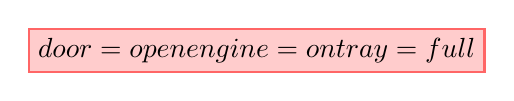
\begin{tikzpicture}[auto]

%
% Styles
%
\tikzstyle{badstate} = [rectangle,draw=red!60,fill=red!20,thick]

\node[badstate] (011) at (  0, 0)  {$\nodd{door=open}{engine=on}{tray=full}$};

\end{tikzpicture}

  \end{center}

\end{frame}
